\documentclass[17pt,a4paper,landscape]{extarticle}
\usepackage[margin=2.35cm,top=0.12cm,left=1.05cm]{geometry}
\usepackage{amsmath}
\usepackage{amssymb}
\usepackage{tasks}
\usepackage{tikz}
\usepackage{xcolor}
\usepackage[sfdefault,lf]{FiraSans}
\renewcommand{\familydefault}{\sfdefault}
\setlength{\parindent}{0pt}
\pagestyle{empty}
\settasks{label=\textbf{\arabic*.}, label-width=2.2em, item-indent=2.95em, column-sep=2.1cm, after-item-skip=4.7em}
\renewcommand{\arraystretch}{1.15}
\everymath{\displaystyle}

\begin{document}
\sffamily
\boldmath

\boldmath

\boldmath

{\LARGE \textbf{Analysing scatter plots (i.e. bivariate) - TARSOG — Foundation}}
\begin{tasks}(3)
\task {Describe the scatter plot using TARSOG.\\[0.4em]
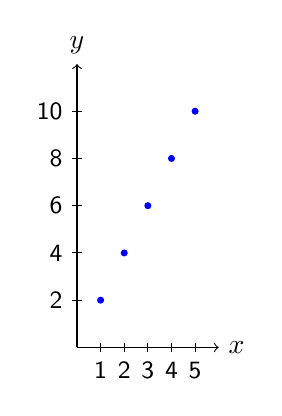
\begin{tikzpicture}[x=0.3cm,y=0.3cm,baseline=(current bounding box.center)]
  \draw[->] (0,0) -- (6,0) node[right] {$x$};
  \draw[->] (0,0) -- (0,12) node[above] {$y$};
  \foreach \x in {1,...,5} \draw (\x,0.2) -- (\x,-0.2) node[below] {\small \x};
  \foreach \y in {2,4,6,8,10} \draw (0.2,\y) -- (-0.2,\y) node[left] {\small \y};
  \fill[blue] (1,2) circle (0.15);
  \fill[blue] (2,4) circle (0.15);
  \fill[blue] (3,6) circle (0.15);
  \fill[blue] (4,8) circle (0.15);
  \fill[blue] (5,10) circle (0.15);
\end{tikzpicture}}
\task {Describe the scatter plot using TARSOG.\\[0.4em]
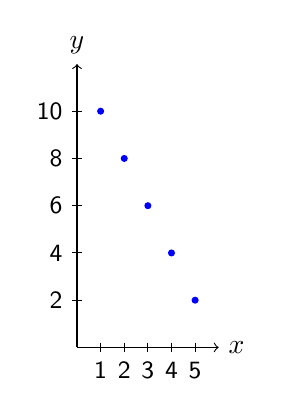
\begin{tikzpicture}[x=0.3cm,y=0.3cm,baseline=(current bounding box.center)]
  \draw[->] (0,0) -- (6,0) node[right] {$x$};
  \draw[->] (0,0) -- (0,12) node[above] {$y$};
  \foreach \x in {1,...,5} \draw (\x,0.2) -- (\x,-0.2) node[below] {\small \x};
  \foreach \y in {2,4,6,8,10} \draw (0.2,\y) -- (-0.2,\y) node[left] {\small \y};
  \fill[blue] (1,10) circle (0.15);
  \fill[blue] (2,8) circle (0.15);
  \fill[blue] (3,6) circle (0.15);
  \fill[blue] (4,4) circle (0.15);
  \fill[blue] (5,2) circle (0.15);
\end{tikzpicture}}
\task {Describe the scatter plot using TARSOG.\\[0.4em]
\begin{tikzpicture}[x=0.3cm,y=0.3cm,baseline=(current bounding box.center)]
  \draw[->] (0,0) -- (6,0) node[right] {$x$};
  \draw[->] (0,0) -- (0,30) node[above] {$y$};
  \foreach \x in {1,...,5} \draw (\x,0.2) -- (\x,-0.2) node[below] {\small \x};
  \foreach \y in {5,10,15,20,25} \draw (0.2,\y) -- (-0.2,\y) node[left] {\small \y};
  \fill[blue] (1,1) circle (0.15);
  \fill[blue] (2,4) circle (0.15);
  \fill[blue] (3,9) circle (0.15);
  \fill[blue] (4,16) circle (0.15);
  \fill[blue] (5,25) circle (0.15);
\end{tikzpicture}}
\task {Identify the trend (linear or non-linear) for each plot above.}
\task {Identify the association (positive or negative) for each plot above.}
\task {Identify the relationship strength (weak, moderate, strong) for each plot above.}
\task {Identify the scatter (constant or non-constant) for each plot above.}
\task {Identify any outliers in the plots above.}
\task {Identify any groupings in the plots above.}
\task {What does TARSOG stand for?}
\task {Match each letter of TARSOG with its meaning.}
\task {Given a scatter plot with a positive linear trend and strong relationship, describe what that means.}
\task {Given a scatter plot with a negative linear trend and moderate relationship, describe what that means.}
\task {Given a scatter plot with a non-linear trend and weak relationship, describe what that means.}
\end{tasks}

\end{document}